% Template for PLoS
% Version 3.5 March 2018
%
% % % % % % % % % % % % % % % % % % % % % %
%
% -- IMPORTANT NOTE
%
% This template contains comments intended
% to minimize problems and delays during our production
% process. Please follow the template instructions
% whenever possible.
%
% % % % % % % % % % % % % % % % % % % % % % %
%
% Once your paper is accepted for publication,
% PLEASE REMOVE ALL TRACKED CHANGES in this file
% and leave only the final text of your manuscript.
% PLOS recommends the use of latexdiff to track changes during review, as this will help to maintain a clean tex file.
% Visit https://www.ctan.org/pkg/latexdiff?lang=en for info or contact us at latex@plos.org.
%
%
% There are no restrictions on package use within the LaTeX files except that
% no packages listed in the template may be deleted.
%
% Please do not include colors or graphics in the text.
%
% The manuscript LaTeX source should be contained within a single file (do not use \input, \externaldocument, or similar commands).
%
% % % % % % % % % % % % % % % % % % % % % % %
%
% -- FIGURES AND TABLES
%
% Please include tables/figure captions directly after the paragraph where they are first cited in the text.
%
% DO NOT INCLUDE GRAPHICS IN YOUR MANUSCRIPT
% - Figures should be uploaded separately from your manuscript file.
% - Figures generated using LaTeX should be extracted and removed from the PDF before submission.
% - Figures containing multiple panels/subfigures must be combined into one image file before submission.
% For figure citations, please use "Fig" instead of "Figure".
% See http://journals.plos.org/plosone/s/figures for PLOS figure guidelines.
%
% Tables should be cell-based and may not contain:
% - spacing/line breaks within cells to alter layout or alignment
% - do not nest tabular environments (no tabular environments within tabular environments)
% - no graphics or colored text (cell background color/shading OK)
% See http://journals.plos.org/plosone/s/tables for table guidelines.
%
% For tables that exceed the width of the text column, use the adjustwidth environment as illustrated in the example table in text below.
%
% % % % % % % % % % % % % % % % % % % % % % % %
%
% -- EQUATIONS, MATH SYMBOLS, SUBSCRIPTS, AND SUPERSCRIPTS
%
% IMPORTANT
% Below are a few tips to help format your equations and other special characters according to our specifications. For more tips to help reduce the possibility of formatting errors during conversion, please see our LaTeX guidelines at http://journals.plos.org/plosone/s/latex
%
% For inline equations, please be sure to include all portions of an equation in the math environment.
%
% Do not include text that is not math in the math environment.
%
% Please add line breaks to long display equations when possible in order to fit size of the column.
%
% For inline equations, please do not include punctuation (commas, etc) within the math environment unless this is part of the equation.
%
% When adding superscript or subscripts outside of brackets/braces, please group using {}.
%
% Do not use \cal for caligraphic font.  Instead, use \mathcal{}
%
% % % % % % % % % % % % % % % % % % % % % % % %
%
% Please contact latex@plos.org with any questions.
%
% % % % % % % % % % % % % % % % % % % % % % % %

\documentclass[10pt,letterpaper]{article}
\usepackage[top=0.85in,left=2.75in,footskip=0.75in]{geometry}

% amsmath and amssymb packages, useful for mathematical formulas and symbols
\usepackage{amsmath,amssymb}

% Use adjustwidth environment to exceed column width (see example table in text)
\usepackage{changepage}

% Use Unicode characters when possible
\usepackage[utf8x]{inputenc}

% textcomp package and marvosym package for additional characters
\usepackage{textcomp,marvosym}

% cite package, to clean up citations in the main text. Do not remove.
% \usepackage{cite}

% Use nameref to cite supporting information files (see Supporting Information section for more info)
\usepackage{nameref,hyperref}

% line numbers
\usepackage[right]{lineno}

% ligatures disabled
\usepackage{microtype}
\DisableLigatures[f]{encoding = *, family = * }

% color can be used to apply background shading to table cells only
\usepackage[table]{xcolor}

% array package and thick rules for tables
\usepackage{array}

% create "+" rule type for thick vertical lines
\newcolumntype{+}{!{\vrule width 2pt}}

% create \thickcline for thick horizontal lines of variable length
\newlength\savedwidth
\newcommand\thickcline[1]{%
  \noalign{\global\savedwidth\arrayrulewidth\global\arrayrulewidth 2pt}%
  \cline{#1}%
  \noalign{\vskip\arrayrulewidth}%
  \noalign{\global\arrayrulewidth\savedwidth}%
}

% \thickhline command for thick horizontal lines that span the table
\newcommand\thickhline{\noalign{\global\savedwidth\arrayrulewidth\global\arrayrulewidth 2pt}%
\hline
\noalign{\global\arrayrulewidth\savedwidth}}


% Remove comment for double spacing
%\usepackage{setspace}
%\doublespacing

% Text layout
\raggedright
\setlength{\parindent}{0.5cm}
\textwidth 5.25in
\textheight 8.75in

% Bold the 'Figure #' in the caption and separate it from the title/caption with a period
% Captions will be left justified
\usepackage[aboveskip=1pt,labelfont=bf,labelsep=period,justification=raggedright,singlelinecheck=off]{caption}
\renewcommand{\figurename}{Fig}

% Use the PLoS provided BiBTeX style
% \bibliographystyle{plos2015}

% Remove brackets from numbering in List of References
\makeatletter
\renewcommand{\@biblabel}[1]{\quad#1.}
\makeatother



% Header and Footer with logo
\usepackage{lastpage,fancyhdr,graphicx}
\usepackage{epstopdf}
%\pagestyle{myheadings}
\pagestyle{fancy}
\fancyhf{}
%\setlength{\headheight}{27.023pt}
%\lhead{
\includegraphics[width=2.0in]{PLOS-submission.eps}}
\rfoot{\thepage/\pageref{LastPage}}
\renewcommand{\headrulewidth}{0pt}
\renewcommand{\footrule}{\hrule height 2pt \vspace{2mm}}
\fancyheadoffset[L]{2.25in}
\fancyfootoffset[L]{2.25in}
\lfoot{\today}

%% Include all macros below

\newcommand{\lorem}{{\bf LOREM}}
\newcommand{\ipsum}{{\bf IPSUM}}





\usepackage{forarray}
\usepackage{xstring}
\newcommand{\getIndex}[2]{
  \ForEach{,}{\IfEq{#1}{\thislevelitem}{\number\thislevelcount\ExitForEach}{}}{#2}
}

\setcounter{secnumdepth}{0}

\newcommand{\getAff}[1]{
  \getIndex{#1}{}
}

\providecommand{\tightlist}{%
  \setlength{\itemsep}{0pt}\setlength{\parskip}{0pt}}

\begin{document}
\vspace*{0.2in}

% Title must be 250 characters or less.
\begin{flushleft}
{\Large
\textbf\newline{Cranium} % Please use "sentence case" for title and headings (capitalize only the first word in a title (or heading), the first word in a subtitle (or subheading), and any proper nouns).
}
\newline
% Insert author names, affiliations and corresponding author email (do not include titles, positions, or degrees).
\\
Ziwei (Crystal) Zang\textsuperscript{\getAff{Smith College}},
Yujia (Emma) Ning\textsuperscript{\getAff{Smith College}},
Kalynn Kosyka\textsuperscript{\getAff{Smith College}}\\
\bigskip
\textbf{\getAff{}}Statistical and Data Sciences, Northampton, MA\\
\bigskip
\end{flushleft}
% Please keep the abstract below 300 words
\section*{Abstract}
Collaborated with the Barresi Lab, we continued \(\Delta\) SCOPE by
extending functionalities in R package--Cranium. We modified existed
functions in Cranium, built new functions and optimized parameters so
that evaluating sample alignments is no longer vulnerable to subjective
biases. Additionally, alignments will be able to run automatically
without labor-intensive manual correction that would introduce more
researcher biases.

% Please keep the Author Summary between 150 and 200 words
% Use first person. PLOS ONE authors please skip this step.
% Author Summary not valid for PLOS ONE submissions.
\section*{Author summary}
This is our first draft.

\linenumbers

% Use "Eq" instead of "Equation" for equation citations.
\hypertarget{introduction}{%
\section{Introduction}\label{introduction}}

The current study serves as an enhancement to Dr.~Michael Barresi's
research at Smith College on categorizing zebrafish brains. The goal of
his research is to use the commissure, an axonal bridge formed to
connect the two hemispheres of the brain, to classify whether a certain
zebrafish belongs to wild type or mutant group.

\begin{figure}
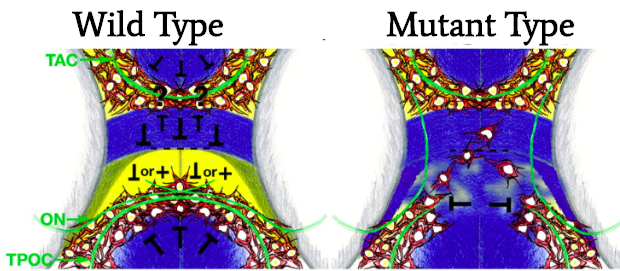
\includegraphics[width=0.9\linewidth]{visualization_paper/wt_yt} \caption{Wild Type and Mutant Commissure}\label{fig:Figure1}
\end{figure}

The difference between wildtype and you-too is shown above. Wild type
zebrafish has a smooth parabolic-shaped commissure, where as in mutant
(you-too) zebrafish, the commissure is either not fully developed or
highly distorted.

During the classification process, instead of following a systematic
approach, Dr.~Barresi's lab could only perform categorization based on
empirical knowledge. As a result, Morgan Schwartz, a former lab member
wrote a Python program called deltascope to: 1. Align crooked 3D
biological images so they could compare between samples; 2. Generate
descriptive graphs with sample statistics; 3. Classify samples into
either wild type or mutant group based on the statistics{[}1{]} {[}2{]}.
Our goal is to ``transfer'' the Python program into R while maintaining
and improving as many features as possible. We modified existed
functions in Cranium package, built new functions and optimized
parameters so that evaluating sample alignments is no longer vulnerable
to subjective biases. Additionally, alignments will be able to run
automatically without labor-intensive manual correction that would
introduce more researcher biases.

\hypertarget{data}{%
\section{Data}\label{data}}

We received our data from Dr.~Jake Schnabl: 43 wild type samples and 35
mutant samples. The data files are in HDF5 (.h5) format. The data points
stored within those files are marked using by fluorescence microscopy,
indicating neuronal signals. The data is processed by an open-source
software, Ilastik, before being read into R. We are working with the
data after processed in Ilastik.

Raw image data was processed in Illastik. Each sample is composed of
data points, which are pixels of the image. Each pixel has a frequency,
which represents the probability of being a real signal. Each data point
in our dataset represents one signal, and the signals have different
frequencies.

\hypertarget{methods}{%
\section{Methods}\label{methods}}

\hypertarget{programming-languages}{%
\subsection{Programming Languages}\label{programming-languages}}

In this study, we used R in order to run algorithms, manipulate data,
and generate visualizations. For accessibility and reproducibility of
this research, we have stored our work on Github. {[}3{]}

\hypertarget{package-cranium}{%
\subsection{\texorpdfstring{Package
\texttt{Cranium}}{Package Cranium}}\label{package-cranium}}

The package \texttt{Cranium} contains several major functionalities
listed below:

\hypertarget{api}{%
\subsubsection{1. API}\label{api}}

The sample datasets for You Too and Wild Type are saved as *.h5 files.
In order to share the data efficiently amongst users, the data is hosted
on Amazon s3 with a readonly link to each sample. Rather than users
individually grabbing each sample, there were functions created in the
cranium R package that allows users to download a bundle of samples per
type (i.e., You Too and Wild Type). Each function downloads all existing
files onto the user's machine in a designated folder the user decides in
addition to outputting the list of samples of type brain class. Prior to
these new functions, the Barresi lab had to share the samples through a
hard drive, thus the new features solve the issue on how to share data
efficiently.

\hypertarget{tidy-data-and-threshold}{%
\subsubsection{2. Tidy Data and
Threshold}\label{tidy-data-and-threshold}}

After reading in the data, tidy function not only converts the original
data to x, y, z coordinates of each signal, but also includes the
signal's frequency. Now the data is assigned as a tidy brain class.

Frequency represents the probability of each pixel being a real signal.
We want to include as many ``real'' signals as possible while getting
rid of signals that are very likely to be ``background noise.'' To do
this, we tested different thresholds and examined model fit. Signals
with frequency lower than the threshold are pruned out, leaving us with
``real'' signals in our data. For example, before we attempted to
optimize threshold level, deltascope treated 0.9 as the standard
threshold. After setting the threshold, individual signals undergo a
binary classification procedure: signals that have frequencies higher
than 0.9 are considered as ``real'' signals whereas signals that have
frequencies lower than 0.9 are pruned out as ``background noise.''

We tested different thresholds for both wild type and mutant (you-too),
separately. Since wild type commissures more or less follow a parabolic
pattern, setting a high threshold would not result in too few data
points (i.e., signals). However, setting a high threshold for mutant
type data would result in a very restricted sample size, thus increasing
the chance of our model overfitting the data. At the same time, setting
a low threshold for mutant type data, while increases the sample size,
allows more noise to creep into the dataset.

\hypertarget{principal-component-analysis-transformation}{%
\subsubsection{3. Principal Component Analysis
Transformation}\label{principal-component-analysis-transformation}}

We can't ensure the samples are mounted exactly the same. Therefore, the
pictures taken are of different angles and coordinates. In order for us
to do further analyses and compare between samples, we need to re-orient
them using Principal Component Analysis (PCA) and identify a consistent
set of axes across all samples. PCA assigns the axis with the most
amount of variation as PC1 (first principal component), the axis with
the second-most variation as PC2, and the axis with least amount of
variation as PC3. Since we are performing the PCA in a 3D space, PCA
would output three 2D planes from three perspectives: xy; yz; xz planes.
For the commissure, we would get 3 views: lateral; dorsal/ventral;
anterior/posterior. We set x axis as the lateral, y axis as the
anterior/posterior, and z as the dorsal/ventral.

\hypertarget{qmodel}{%
\subsubsection{4. Qmodel}\label{qmodel}}

We built the Qmodel function to fit a quadratic model to the data in
order to capture the shape of the commissure as well as evaluating model
fit. The quadratic model fits on the xy plane. Our goal is to have the
best model fit. Qmodel outputs model statistics including: \(r^2\) ,
adjusted \(r^2\) , sigmal (RSE), statistic, p.value, df, logLik, AIC,
BIC, deviance, df.residual, num.signal, quad.coeff, RMSE. \#\#\# \(r^2\)
: Also called the coefficient of determination or the coefficient of
multiple determination for multiple regression. \(r^2\) ranges from 0 to
1. It is calculated from the variance explained by the model divided by
total variance. Higher \(r^2\) values represent smaller differences
between the observed data and the fitted values, indicating a better fit
of the model. Note that \(r^2\) is a relative scale of model fit.

\hypertarget{adjusted-r2}{%
\subsubsection{\texorpdfstring{Adjusted \(r^2\)
:}{Adjusted r\^{}2 :}}\label{adjusted-r2}}

Based on \(r^2\) , adjusted \(r^2\) --adjusts for the number of terms in
the model, the degrees of freedom.

\hypertarget{rmse-root-mean-squared-error}{%
\subsubsection{RMSE (Root Mean Squared
Error)}\label{rmse-root-mean-squared-error}}

gives the difference between observed data and model's predicted values.
Lower RMSE values represent smaller difference between observed data and
model's predicted values.

\hypertarget{sigma}{%
\subsubsection{Sigma}\label{sigma}}

It is the square root of the estimated variance of the residuals

\hypertarget{statistic}{%
\subsubsection{Statistic}\label{statistic}}

A piece of data that is related to a larger set of data

\hypertarget{p.value}{%
\subsubsection{P.value}\label{p.value}}

It is the probability that chance alone would produce a test statistic
as extreme as the observed test statistic.

\hypertarget{df}{%
\subsubsection{Df}\label{df}}

Degrees of freedom

\hypertarget{loglik}{%
\subsubsection{logLik}\label{loglik}}

A function in R that determines the log likelihood of a fitted model.

\hypertarget{aic}{%
\subsubsection{AIC}\label{aic}}

Akaike information criterion represents the estimate in quality of model
relative to other models.

\hypertarget{bic}{%
\subsubsection{BIC}\label{bic}}

Bayesian information criterion (BIC) or Schwarz information criterion

\hypertarget{deviance}{%
\subsubsection{Deviance}\label{deviance}}

A value of goodness-of-fit for a statistical model.

\hypertarget{df.residual}{%
\subsubsection{df.residual}\label{df.residual}}

Residual degree of freedom

\hypertarget{num.signal}{%
\subsubsection{num.signal}\label{num.signal}}

It gives the number of signals being captured for the sample after
filter out the signals that are less than the threshold.

\hypertarget{quad.coeff}{%
\subsubsection{Quad.coeff}\label{quad.coeff}}

The quadratic coefficient of the model \(y=x^2+x\).

\hypertarget{linear-model}{%
\subsubsection{5. Linear Model}\label{linear-model}}

A good PCA transformation will result in mean z value to be zero. Thus,
we build linear model \(z=0\) to evaluate the PCA transformation.
Visually, we will observe the line at \(z=0\) on the xz plane and yz
plane if PCA is transformed correctly. A bad fitted linear model is
indicated by having a curvature in the xz plane and yz plane, which
could cause by rotation around x axis or an incorrectly selected PC1
(first principal component).

\hypertarget{plotting}{%
\subsubsection{6. Plotting}\label{plotting}}

\hypertarget{results}{%
\section{Results}\label{results}}

\hypertarget{threshold-optimization-evaluation}{%
\subsection{1. Threshold optimization
evaluation}\label{threshold-optimization-evaluation}}

\hypertarget{wild-type}{%
\subsubsection{Wild Type}\label{wild-type}}

For wild type sample, we tested threshold 24 different threshold:
threshold = \{0.6, 0.62, 0.64, 0.66, 0.69, 0.7, 0.72, 0.75, 0.78, 0.8,
0.81, 0.82, 0.83, 0.84, 0.85, 0.86, 0.87, 0.88, 0.90, 0.91, 0.92, 0.93,
0.96, 0.99\}. Next, we fit the qmodel to each sample and for each
threshold value. We are able to find the threshold for each sample that
gives the highest adjusted \(r^2\) . 4 (16.3\%) sample achieved their
highest adjusted \(r^2\) when setting threshold 0.87; 11 (25.6\%)
samples achieved their highest adjusted \(r^2\) when setting threshold
0.9; 6 (14.0\%) samples achieved their highest adjusted \(r^2\) when
setting threshold 0.92; 9 (20.9\%) samples achieved their highest
adjusted \(r^2\) when setting threshold 0.93. Boxplots in Figure 2 show
the adjusted \(r^2\) for each threshold value. We had good model fit for
all thresholds, and the mean adjusted \(r^2\) is 0.9. The adjusted
\(r^2\) is slightly higher for threshold 0.87 and 0.9. Thus, we conclude
that the range of optimal thresholds for wild type is between 0.87 and
0.9

\begin{figure}
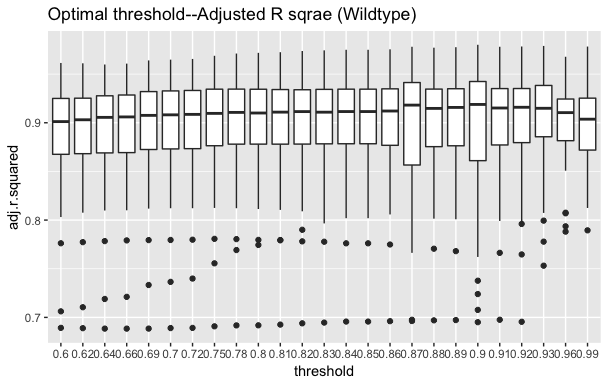
\includegraphics[width=0.9\linewidth]{visualization_paper/threshold_boxplot_wt} \caption{Optimal threshold--Adjusted r2 (Wild Type)}\label{fig:Figure2}
\end{figure}

\hypertarget{mutant}{%
\subsubsection{Mutant}\label{mutant}}

For mutant sample, we tested 29 different thresholds: threshold = \{0.4,
0.42, 0.44, 0.46, 0.48, 0.5, 0.52, 0.54, 0.56, 0.58, 0.6, 0.62, 0.64,
0.66, 0.7, 0.75, 0.8, 0.81, 0.82, 0.83, 0.84, 0.85, 0.86, 0.87, 0.88,
0.89, 0.9, 0.91, 0.92\}. Next, we fit the qmodel to each sample and for
each threshold value. We are then able to find the optimal threshold for
each sample that gives the highest adjusted \(r^2\) value. According to
Figure 2, x-axis is showing different thresholds and y-axis gives us the
adjusted \(r^2\) . Each line represents a mutant sample. The range of
the adjusted \(r^2\) is very large, indicating large number of samples
having poor model fit.

According to Figure 3, we show the boxplots of adjusted \(r^2\) for each
threshold value. Changing threshold is not improving model fit
significantly. Thus we can't conclude an optimal threshold for the
mutant samples.

\begin{figure}
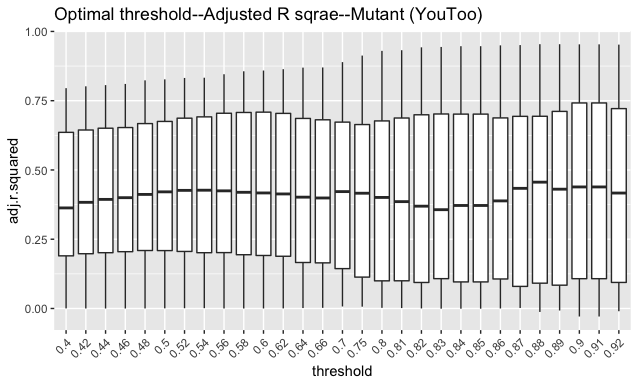
\includegraphics[width=0.9\linewidth]{visualization_paper/threshold_boxplot_yt} \caption{Optimal threshold--Adjusted r2--Mutant(You Too)}\label{fig:Figure3}
\end{figure}

\hypertarget{threshold-optimization}{%
\subsubsection{Threshold Optimization}\label{threshold-optimization}}

And then we compared model fit of wild type and mutant sample by
comparing their average adjusted \(r^2\) for each threshold. For each
threshold, we computed the average adjusted \(r^2\) for 43 wild type
samples and the average adjusted \(r^2\) for 35 mutant samples. As shown
in Figure 4, x-axis represents the average adjusted \(r^2\) for wild
type and the y-axis represents the average adjusted \(r^2\) for mutant
type. A perfect model fit will have x=1 and y=1, and our goal is to
identify the point that has the smallest Euclidean distance to (1,1).

\begin{figure}
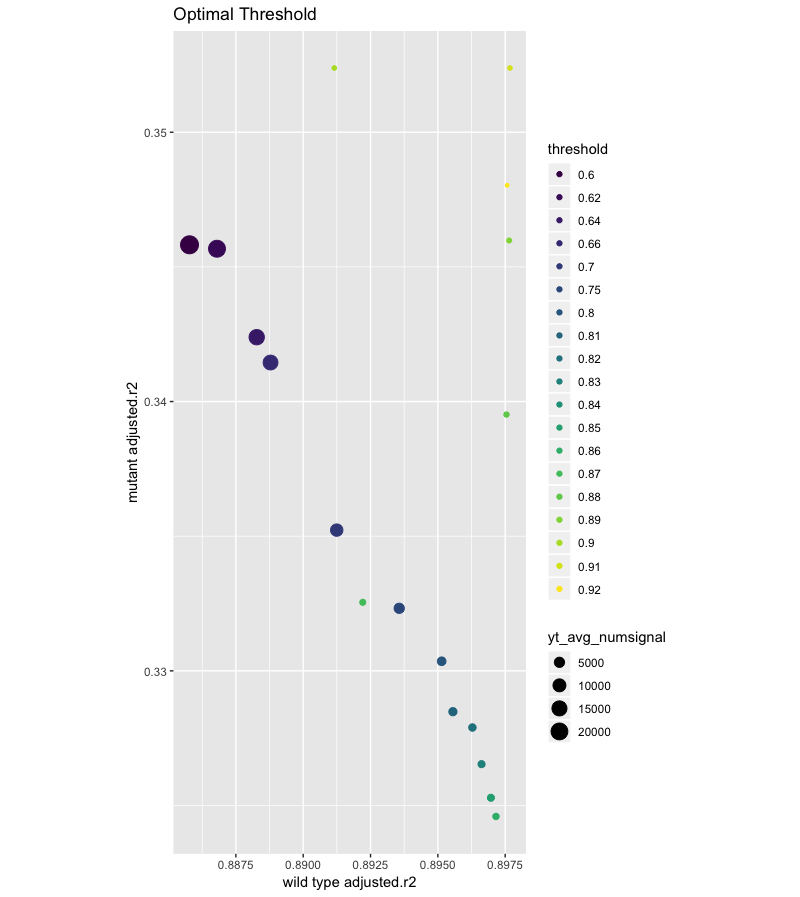
\includegraphics[width=1\linewidth]{visualization_paper/optimal_threshold} \caption{Optimal Threshold}\label{fig:Figure4}
\end{figure}

\hypertarget{pca-transformation-model-fit-evaluation}{%
\subsection{2. PCA Transformation Model Fit
Evaluation}\label{pca-transformation-model-fit-evaluation}}

We compared the adjusted \(r^2\) of the model before and after PCA
transformation, and found out that PCA transformation significantly
improved the model fit.

\hypertarget{wild-type-1}{%
\subsubsection{Wild Type}\label{wild-type-1}}

We performed paired sample t-test on the wild type samples by setting
default threshold 0.9. As shown in Figure 5, the x-axis shows the
adjusted \(r^2\) before the PCA reorientation, and y-axis shows the
adjusted \(r^2\) after the PCA reorientation. Each point represents a
signal in the wild type sample. It was found that the average adjusted
\(r^2\) after PCA transformation is significantly higher than the
average adjusted \(r^2\) before PCA transformation with a p-value
=\(5.765^{-10}\). The result ensures the importance of PCA
transformation.\\

\begin{figure}
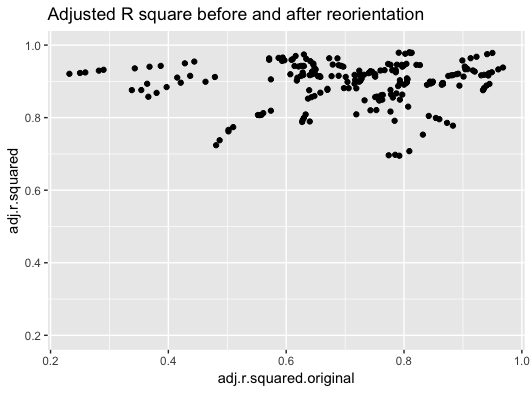
\includegraphics[width=0.9\linewidth]{visualization_paper/r2_ro_comparison_wt} \caption{Adj. r2 before and after PCA reorientation (wild type)}\label{fig:Figure5}
\end{figure}

\hypertarget{mutant-1}{%
\subsubsection{Mutant}\label{mutant-1}}

We performed paired sample t-test on the wild type sample by setting
optimal threshold 0.8. As shown in Figure 6, the x-axis shows the
adjusted \(r^2\) before the PCA reorientation, and y-axis shows the
adjusted \(r^2\) after the PCA reorientation. Each point represents a
signal in the mutant sample.It was found that the average adjusted
\(r^2\) after PCA transformation is significantly higher than the
average adjusted \(r^2\) before PCA transformation with a p-value =
\(1.863^{-4}\). The result ensures the importance of PCA transformation.

\begin{figure}
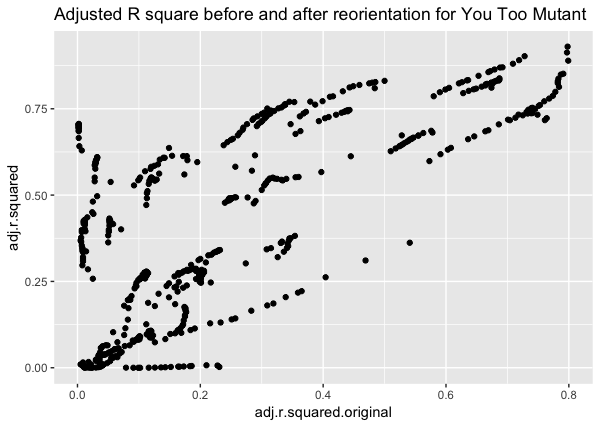
\includegraphics[width=0.9\linewidth]{visualization_paper/r2_ro_comparison_yt} \caption{Adj. r2 before and after PCA reorientation (mutant)}\label{fig:Figure6}
\end{figure}

\hypertarget{references}{%
\section*{References}\label{references}}
\addcontentsline{toc}{section}{References}

\hypertarget{refs}{}
\leavevmode\hypertarget{ref-Schwartz18}{}%
1. M. Schwartz BB J. Schnab. A new computational method to quantify
3D383image data and to detail changes in morphological structure and
spatial384relationships during nervous system development. 2018;

\leavevmode\hypertarget{ref-Hu18}{}%
2. S. Hu DT W. Li. Classification of wild type and mutant zebrafish
brains viaComputational method. 2018;

\leavevmode\hypertarget{ref-rticles19}{}%
3. Allaire J, Xie Y, R Foundation, Wickham H, Journal of Statistical
Software, Vaidyanathan R, et al. Rticles: Article formats for r markdown
{[}Internet{]}. 2019. Available:
\url{https://CRAN.R-project.org/package=rticles}

\nolinenumbers


\end{document}

